\documentclass[twoside]{article}
\usepackage{aistats2016}
\usepackage{graphicx}
\graphicspath{{picF/}}
\usepackage{amsmath,amssymb,amsbsy,amsfonts,amsthm}
\usepackage{tikz}
\usetikzlibrary{arrows,decorations.pathmorphing,backgrounds,positioning,fit}

\newcommand{\vvmK}{\dot{\eta}}
\newcommand{\vvmW}{\dot{\zeta}}
\newcommand{\vvmDK}{\dot{\alpha}}
\newcommand{\vvmKW}{\dot{\beta}}
\newcommand{\vvmbDK}{\bar{\alpha}}
\newcommand{\vvmbKW}{\bar{\beta}}
\newcommand{\vvmDWK}{\mu}
\newcommand{\pmK}{\eta}
\newcommand{\pmW}{\zeta}
\newcommand{\vmK}{\alpha}
\newcommand{\vmW}{\beta}
\newcommand{\vmDK}{\theta}
\newcommand{\vmKW}{\phi}

\newcommand{\pr}{\mathbf{p}}
\newcommand{\dd}{\mathbf{d}}
\newcommand{\divergence}{\mathbb{K}}
\newcommand{\entropy}{\mathbb{H}}
\newcommand{\expectation}{\mathbb{E}}
\newcommand{\carac}[1]{\mathbb{I}[{#1}]}
\newcommand{\mbeta}{\mathbf{Boojum}}
\newcommand{\cpnt}[2]{{#1}^{(\!{#2}\!)}}
\newcommand{\assignn}{\longleftarrow}
\newcommand{\assign}[1]{\underset{\textbf{[#1]}}{\longleftarrow}}
\newcommand{\ruleref}[1]{\textbf{[#1]}}

\newtheorem{definition}{Definition}
\newtheorem{lemma}{Lemma}
\newtheorem{proposition}{Proposition}

\tikzset{BNVar/.style={circle,draw}}
\tikzset{BNVarDiscrete/.style={rectangle,draw}}
\tikzset{BNObserved/.style={fill=black!15}}


% If your paper is accepted, change the options for the package
% aistats2016 as follows:
%
%\usepackage[accepted]{aistats2016}
%
% This option will print headings for the title of your paper and
% headings for the authors names, plus a copyright note at the end of
% the first column of the first page.


\begin{document}

% If your paper is accepted and the title of your paper is very long,
% the style will print as headings an error message. Use the following
% command to supply a shorter title of your paper so that it can be
% used as headings.
%
%\runningtitle{I use this title instead because the last one was very long}

% If your paper is accepted and the number of authors is large, the
% style will print as headings an error message. Use the following
% command to supply a shorter version of the authors names so that
% they can be used as headings (for example, use only the surnames)
%
%\runningauthor{Surname 1, Surname 2, Surname 3, ...., Surname n}

\twocolumn[

\aistatstitle{A fully Bayesian view of Latent Dirichlet Allocation }

\aistatsauthor{ Anonymous Author 1 \And Anonymous Author 2 \And Anonymous Author 3 }

\aistatsaddress{ Unknown Institution 1 \And Unknown Institution 2 \And Unknown Institution 3 } ]

\begin{abstract}
    Abstract...
\end{abstract}


\section{Introduction}
\section{Related work}

The LDA model \cite{blei_latent_2003} has been extended in many different ways to address different problems. Information about document authorship has, for example, been added to the model in \cite{Rosen_Zvi_2004}, whereas the integration of correlations between topics in the model has been explored in \cite{blei_correlated_2007}; more recently, \cite{Boyd_Graber_2009} describes an extension to model multilingual unaligned collections. Other extensions have focused on streaming or online versions of the model: \cite{Yao_2009} focuses on efficient methods for inference in streaming collections, whereas \cite{Wang_2012} introduces a new model for text streams based on transition probabilities between topics of successive documents and \cite{hoffman_online_2010} proposes an online variational Bayes algorithm for LDA based on mini-batches.




\section{A conjugate prior for the Dirichlet distribution}
It is well known that the exponential family of distributions satisfies important stability properties, which lead to elegant, analytical expressions in Bayesian inference, hence its massive use in Bayesian models. One property is that any distribution in that family has a natural conjugate also in that family, and there is a systematic procedure to compute it. For example, the Dirichlet distribution can be derived in this way as a conjugate to the multinomial distribution, and they are both in the exponential family. In the sequel, we are interested in a conjugate to the Dirichlet itself, which is easy to derive by application of the same systematic procedure. We name it here the $\mbeta$ distribution\footnote{a.k.a. the Snark distribution, because the Snark is a Boojum, you see.}, for lack of a better name. It is a distribution over the positive orthant $\mathbb{R}_+^N$ (the parameter space of the $N$-dimensional Dirichlet), and has two parameters $m,\boldsymbol{\tau}$ where $m\in\mathbb{R}$ is a scalar and $\boldsymbol{\tau}\in\mathbb{R}^N$ is a vector (as a general rule, the parameter space of the conjugate has dimension one plus the dimension of the parameter space of the original distribution). It is defined, for $\boldsymbol{x}\in\mathbb{R}_+^N$ by
\begin{eqnarray}
\mbeta(\boldsymbol{x};m,\boldsymbol{\tau}) & \triangleq & \frac{1}{Z(m,\boldsymbol{\tau})}\mathcal{B}(\boldsymbol{x})^m\exp-\boldsymbol{\tau}\boldsymbol{x}
\end{eqnarray}
where $\mathcal{B}$ denotes the multivariate beta function $\mathcal{B}(\boldsymbol{x})\triangleq\frac{\prod_n\Gamma(x_n)}{\Gamma(\sum_nx_n)}$ which is also the normalising constant of the Dirichlet distribution with parameter $\boldsymbol{x}$, and $Z(m,\boldsymbol{\tau})$ is the normalising constant of the $\mbeta$ distribution itself, defined by
\begin{eqnarray*}
Z(m,\boldsymbol{\tau}) & \triangleq & \int_{\boldsymbol{x}\in\mathbb{R}_+^N}\mathcal{B}(\boldsymbol{x})^m\exp-\boldsymbol{\tau} \boldsymbol{x}\;\dd{\boldsymbol{x}}
\end{eqnarray*}
The expression $\boldsymbol{\tau} \boldsymbol{x}$ in the definition denotes the scalar product of the two vectors. Of course, for the distribution to be proper, the normalising constant must be finite, which is not always the case. Although no analytical formula is known for $Z(m,\boldsymbol{\tau})$, one exists for its finiteness:
\begin{proposition}
\label{prop:mbeta-proper}
The distribution $\mbeta(m,\boldsymbol{\tau})$ is proper, i.e. $Z(m,\boldsymbol{\tau})<\infty$, if and only if\footnote{For any whole number $N$, we use the shorthand $n\in N$ to mean $n\in\{1\ldots N\}$}
\[
\begin{array}{l}
\forall n\in N\;\tau_n>0 \;\textrm{ and }\; m<1 \;\textrm{ and }\\
(m\geq0 \;\textrm{ or }\; \sum_{n\in N}\exp-\frac{\tau_n}{|m|}<1)
\end{array}
\]
\end{proposition}
Now, conjugacy with the Dirichlet distribution is expressed by the following property.
\begin{proposition}
Let $(\boldsymbol{y}_p)_{p\in P}$ be a family of random variables over the simplex of $\mathbb{R}_+^N$, which are mutually independent given a random variable $\boldsymbol{x}$ over $\mathbb{R}_+^N$. We have
\[
\begin{array}{l}
\begin{array}{ll}
\textrm{Prior:} & \boldsymbol{x} \sim \mbeta(m,\boldsymbol{\tau})\\
\textrm{Observation:} & \forall p\in P\;\boldsymbol{y}_p|\boldsymbol{x} \sim \mathbf{Dirichlet}(\boldsymbol{x})\\
\Longrightarrow
\textrm{Posterior:} &
\boldsymbol{x}|(\boldsymbol{y}_p)_{p\in P} \sim \mbeta(m',\boldsymbol{\tau}')
\end{array}\\
\textrm{where } m'=m-|P|\;\;\boldsymbol{\tau}'=\boldsymbol{\tau}-\sum_{p\in P}\log\boldsymbol{y}_p
\end{array}
\]
This holds whenever the prior is proper, in which case so is the posterior.
\end{proposition}
%%%%%%%%%%%%%%%%%%%%%%%%%%%%%%%%%%%%%%%%%%%%%%%%%%%%%%%%%%%%%%%%%%%%%%%%%%%
\section{The LDA model revisited}
%%%%%%%%%%%%%%%%%%%%%%%%%%%%%%%%%%%%%%%%%%%%%%%%%%%%%%%%%%%%%%%%%%%%%%%%%%%
\begin{figure*}
\begin{tabular}{c@{\hspace{1cm}}c}
\begin{minipage}{6cm}
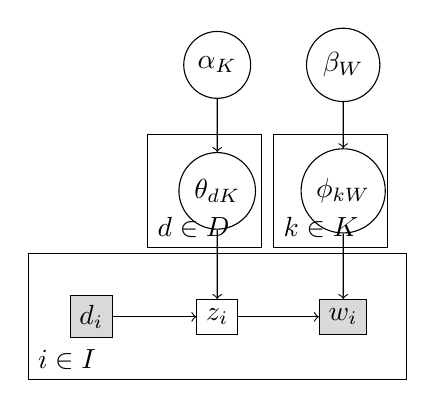
\begin{tikzpicture}[scale=.8]
\node (d) at (0,0) [BNVarDiscrete,BNObserved] {$d_i$};
\node (z) at (2,0) [BNVarDiscrete] {$z_i$};
\node (w) at (4,0) [BNVarDiscrete,BNObserved] {$w_i$};
\node (theta) at (2,2) [BNVar] {$\vmDK_{dK}$};
\node (phi) at (4,2) [BNVar] {$\vmKW_{kW}$};
\node (alpha) at (2,4) [BNVar] {$\vmK_K$};
\node (beta) at (4,4) [BNVar] {$\vmW_W$};
\draw [->] (d) -- (z);
\draw [->] (z) -- (w);
\draw [->] (alpha) -- (theta);
\draw [->] (theta) -- (z);
\draw [->] (beta) -- (phi);
\draw [->] (phi) -- (w);
\draw (-1,-1) rectangle (5,1);
\draw (-1,-1) node[above right] {$i\in I$};
\draw (.9,1.1) rectangle (2.7,2.9);
\draw (.9,1.1) node[above right] {$d\in D$};
\draw (2.9,1.1) rectangle (4.7,2.9);
\draw (2.9,1.1) node[above right] {$k\in K$};
\end{tikzpicture}
\end{minipage} &
$
\begin{array}{l}
\begin{array}{l}
p(\vmK_K\vmW_W\vmDK_{DK}\vmKW_{KW}z_Iw_I|d_I) =\\
\hspace{1cm}p(\vmK_K)p(\vmW_W)\\
\hspace{1cm}\prod_{d\in D}p(\vmDK_{dK}|\vmK_K)\prod_{k\in K}p(\vmDK_{kW}|\vmW_W)\\
\hspace{1cm}\prod_{i\in I}p(z_i|d_i\vmDK_{DK})p(w_i|z_i\vmKW_{KW})
\end{array}
\vspace{.3cm}
\\
\begin{array}{rcl@{\hspace{.5cm}}rcl}
\vmK_K & \sim & \cpnt{p}{K} & \vmW_W & \sim & \cpnt{p}{W}
\end{array}
\\
\begin{array}{r@{\hspace{.5cm}}rcl}
\forall d\in D & \vmDK_{dK}|\vmK_K & \sim & \mathbf{Dirichlet}(\vmK_K)\\
\forall k\in K & \vmKW_{kW}|\vmW_W & \sim & \mathbf{Dirichlet}(\vmW_W)\\
\forall i\in I & z_i|d_i\vmDK_{DK} & \sim & \mathbf{Cat}(\vmDK_{d_iK})\\
\forall i\in I & w_i|z_i\vmKW_{KW} & \sim & \mathbf{Cat}(\vmKW_{z_iW})
\end{array}
\end{array}
$
\end{tabular}
\begin{eqnarray}
\label{eqn:logprobtrue}
\log p(\vmK_K\vmW_W\vmDK_{DK}\vmKW_{KW}z_I|w_Id_I) & = &
\log\cpnt{p}{K}(\vmK_K)+\log\cpnt{p}{W}(\vmW_W)-D\log\mathcal{B}(\vmK_K)-K\log\mathcal{B}(\vmW_W)\\
\nonumber & + & \sum_{dk}(\vmK_k{-}1)\log\vmDK_{dk}+\sum_{kw}(\vmW_w{-}1)\log\vmKW_{kw}+\sum_{ik}\carac{z_i=k}(\log\vmDK_{d_ik}{+}\log\vmKW_{kw_i})
\end{eqnarray}
\caption{\label{fig:fullbn}The full Bayesian network of the LDA model and the decomposition of its joint distribution $q$.}
\end{figure*}
Given a number $D$ of documents, $W$ of words (or terms), $K$ of topics and $I$ of occurrences, a realisation consists of the following random variables\footnote{In the sequel, we take the convention of not distinguishing the vectors by typesetting them in boldface, but rather by systematically recalling their index ranges as subscripts.}: $(i)$ a tuple $(d_i,z_i,w_i)_{i\in I}$, where for each $i\in I$, the discrete objects $d_i\in D,z_i\in K,w_i\in W$ denote, respectively, the document, the topic and the word associated with occurrence $i$; $(ii)$ two stochastic matrices $\vmDK_{DK}$ (of dimension $D\times K$) and $\vmKW_{KW}$ (of dimension $K\times W$) which characterise each document $d$ as the distribution of topics $\vmDK_{dK}$ and each topic $k$ as the distribution of words $\vmKW_{kW}$; $(iii)$ two positive vectors $\vmK_K$ and $\vmW_W$ which characterise the topics and words of the whole collection.

The space of realisations is that of complete collections of documents: this explains why the collection-level variables $\vmK_K$ and $\vmW_W$ are random, and not parameters. Besides the known size parameters $D,W,K,I$, the model has two possibly unknown parameters $\cpnt{p}{K}$ and $\cpnt{p}{W}$, which are distributions for $\vmK_K$ and $\vmW_W$, respectively. For the sake of symmetry, the occurrence-document vector $d_I$ is considered a random variable, but it is assumed always observed and independent of all the rest, so it could as well have been treated as a known parameter. All probability expressions are conditioned upon it. The full graphical representation of the LDA model is given in Figure~\ref{fig:fullbn}. Conditioned to the observation of the occurrence-word vector $w_I$, the log probability is given, up to some additive constant depending only on $d_I,w_I$, by~(\ref{eqn:logprobtrue}).

Note that, at this point, we make no assumption on the distributions $\cpnt{p}{K}$ and $\cpnt{p}{W}$. Our main contribution is precisely in studying the impact of the choice of these distributions. We show that an appropriate choice leads to a new formulation of the variational approximation of LDA, which we investigate.
\section{Fully variational Bayes for Latent Dirichlet Allocation}
\section{Experiments}

In order to evaluate our model we ran experiments over two corpus to compare the typical LDA and his fully bayesian formulation. We uesd a 20 news groups dataset and a nips 2012 set of articles. Each of them were divided into a training and test set corpus. We fit both a classical LDA model and the full variational LDA using the training set. The test set was used to assert to convergence of the training phase by computing the perplexity of the model. To compute it we follow a fold-in procedure and  use the approximation in (Asuncion, 2009) to compute the perplexity. Hence the topic-word distribution is fit on the learning set and the document-topic distribution is evaluated on the testing set, thus the perplexity of the model is computed as follow: 
\[ \log p(x^{test}) = \sum_{jw} N_{jw} \log \frac{1}{S} \sum_s \sum_k \theta^s_{kj} \phi^s_{wk} \]

Each inference procedure was run over 50 iterations and reproduced 10 times to provide a stability measure. Therefore, the figure shows the mean perplexity for each run and his variance.

\section{Discussion}

\subsubsection*{Acknowledgements}

Use unnumbered third level headings for the acknowledgements.  All
acknowledgements go at the end of the paper.  Be sure to omit any
identifying information in the initial double-blind submission!


\subsubsection*{References}

Asuncion, Arthur, et al. "On smoothing and inference for topic models." Proceedings of the Twenty-Fifth Conference on Uncertainty in Artificial Intelligence. AUAI Press, 2009.

\end{document}
